\chapter{Moving Forward}~\label{chp:moving_forward}
\graphicspath{{figures/moving-forward/}}

% Focus of chapter 2 and how it links to G-SMOTENC
In Chapter~\ref{chp:data-augmentation-trends} we studied the state-of-the-art
in data augmentation algorithms, which was necessary to proceed to subsequent
steps of the work plan. Based on these findings, in
Chapter~\ref{chp:kmeans-smote} we used an oversampling method to address a
know limitation of imbalanced learning in LULC\@. An additional limitation we
found in oversampling methods was the lack of models capable of addressing
datasets with both metric and non-metric features. We plan to address this
limitation by modifying a state-of-the-art oversampling method, based on RQ4,
as described in Subsection~\ref{sec:main_objectives}. This work will be added
as a new Chapter between Chapters~\ref{chp:data-augmentation-trends}
and~\ref{chp:kmeans-smote}. At the time of writing, the algorithmic
implementation, dataset collection and preprocessing, and experimental results
have been completed. The writing of the Chapter is in progress.

The Geometric-SMOTENC oversampler will use the generation mechanism described
in~\cite{Douzas2019}, while encoding the continuous features, calculating the
selected observations' nearest neighbors and generating the categorical
feature values for the synthetic data using the method described
in~\cite{Chawla2002}. This approach allows the usage of a state-of-the-art
oversampling method with categorical features. The experimental results have
shown that G-SMOTENC outperforms the oversamplers compatible with this
type of data (\textit{i.e.}, Random Oversampling and SMOTENC).

% Focus of chapter 4 and 5 and how they introduced individual elements to AL,
% the next step is SAD-Learning: merging the different contributions while
% adding other hybrid learning methods to leverage more information from
% unlabeled data
In Chapters~\ref{chp:al-generator-lulc}
and~\ref{chp:active-learning-augmentation} we modify the AL framework as a
means to address RQ3. However, the work presented can be further enriched with
the application of other methods that leverage information from unlabeled
data, specifically semi-supervised and self-supervised learning techniques to
form a single framework, the Self-Supervised Semi-Supervised Active Deep
Learning (S$^4$AD-Learning) framework.
This work is also under development and is intended to follow
Chapter~\ref{chp:active-learning-augmentation}. At the time of writing, the
algorithmic implementation is in progress.

The conceptualization of the framework discussed is shown in
Figures~\ref{fig:al_initialization2} and~\ref{fig:al_iteration2}. We intend to
use a self-supervised learning technique before the data annotation phase of
AL to have a well-tuned, pretrained model to start with. The iterative process
will use a semi-supervised loss function to train the shallow layers of the
network, to maximize the value of both labeled and unlabeled data in the
iterative process. In addition, the training data will also be augmented
using synthetic data to further train and regularize the classifier.

% \begin{figure}
% 	\centering
% 	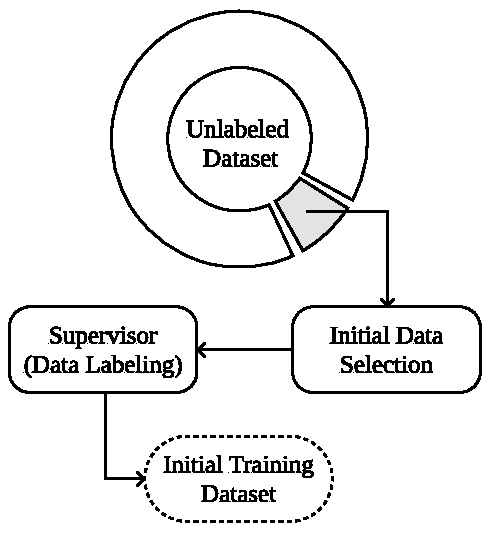
\includegraphics[width=.85\linewidth]{al_initialization}
%     \caption{%
%         Diagram depicting the initialization of the S$^4$AD-Learning model.
%     }~\label{fig:al_initialization2}
% \end{figure}
% 
% 
% \begin{figure}
% 	\centering
% 	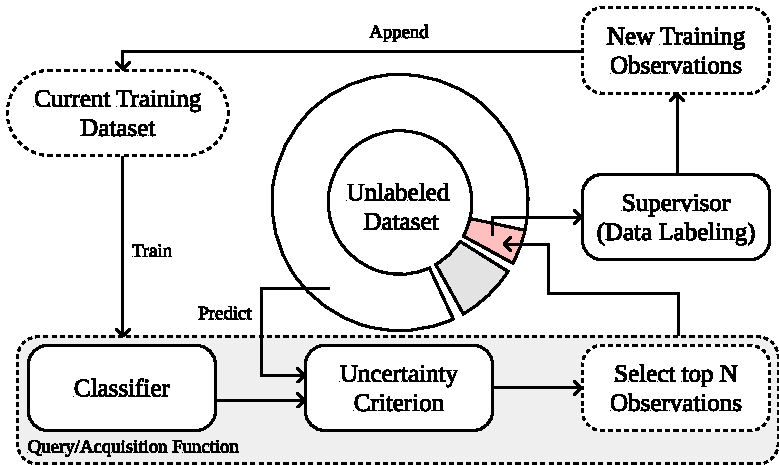
\includegraphics[width=.5\linewidth]{al_iteration}
%     \caption{%
%         Diagram depicting the iterative procedure of the S$^4$AD-Learning model.
%     }~\label{fig:al_iteration2}
% \end{figure}

The last chapter will close the thesis with the conclusions, discussion of the
proposed research questions and recommendations for future work based on the
results presented in previous chapters.
